\documentclass{TDP005mall}

\usepackage{enumitem}
\usepackage{graphicx}
\usepackage{float}


\newcommand{\version}{Version 1.1}
\author{Albin Dahlén, \url{albda746@student.liu.se}\\
Filip Ingvarsson, \url{filin764@student.liu.se}}
\title{Kravspecifikation}
\date{2022-11-21}
\rhead{Albin Dahlén\\
Filip Ingvarsson}



\begin{document}
  \projectpage
  \tableofcontents
  \newpage

  \section{Revisionshistorik}
  \begin{table}[!h]
    \begin{tabularx}{\linewidth}{|l|X|l|}
      \hline
      Ver. & Revisionsbeskrivning & Datum \\\hline
      1.0 & Första utkast & 22-11-14 \\\hline
      1.1 & Förändrat efter semenarie & 22-11-21 \\\hline
    \end{tabularx}
  \end{table}


  \section{Spelidé}
  Spelet kommer utspela sig i en 2D-värld med ett fågelperspektiv.
  Spelet är ett evighets shoot'em up där spelaren styr en karaktär som blir attackerad av vågor med fiender.
  Spelaren har ett projektilvapen som kan skjuta projektiler för att göra skada på fienderna.
  Detta projektilvapen kommer att kunna uppgraderas under spelets gång.
  Det kommer finnas olika typer av fiender där de olika typerna olika hastighet, attackskada, liv och hur de attackerar.
  Under spelets gång ökas svårighetsgraden genom att det kommer fler fiender per våg samt att vågorna kommer oftare.
  Spelet kommer sedan att generera ett highscore beroende på hur många fiender som dödats samt hur många vågor som är avklarade.

  \section{Målgrupp}
  Spelet riktar sig till personer som gillar shoot 'em spel och möjligheten att tävla med andra genom highscores.

  \section{Spelupplevelse}
  Spelet kommer vara utmanande och har stor återspelbarhet där man kan testa olika vapen och olika uppgraderingar.
  Spelet kan även spelas om flera gånger för att försöka slå sitt eget eller sina vänners highscore.

  \section{Spelmekanik}
  Spelaren kommmer röra sig i spelet genom piltangenter, man kan byta dessa knappar i menyn.
  \begin{table}[H]
    \begin{center}
      \begin{tabular}{ |c|c| }
        \hline
        \textbf{Tangentknapp} & \textbf{Åtgärd} \\
        \hline
        → & Flytta spelaren åt höger \\
        \hline
        ↓ & Flytta spelaren neråt \\
        \hline
        ← & Flytta spelaren åt vänster \\
        \hline
        ↑ & Flytta spelaren uppåt \\
        \hline
        Mouse button 1 & Använd vapen \\
        \hline
      \end{tabular}
    \end{center}
    \caption{Keybindings}
    \label{tab:movement}
  \end{table}

  \section{Spelbeskrivning}
  Nedan följer beskrivningar för olika delar av spelet.
  
  \subsection{Spelplan}
  \begin{itemize}
    \item Hinder på spelplanen slumpas fram.
    \item Spelplanen har en fixerad storlek.
  \end{itemize}

  \subsection{Spelare}
  \begin{itemize}
    \item Spelaren är den figur som användaren styr.
    \item Spelaren kan använda sitt vapen för att skada fiendeobjekt.
    \item Spelaren kan röra sig uppåt, neråt, höger och vänster.
    \item Spelaren startar i mitten av spelplanen när spelet startar.
    \item Spelaren börjar med 100 i hälsa.
    \item Spelaren kan kollidera med fiender.
    \item Spelaren kan kollidera med hinder på spelplanen.
    \item Spelaren förlorar hälsa vid kollision med en fiende.
    \item Spelaren kan inte röra sig utanför spelplanen.
    \item När spelaren har 0 eller mindre i hälsa avslutas spelet.
  \end{itemize}


  \subsection{Fiendetyper}
  Nedan följer beskrivningar av olika fiendetyper som finnas i spelet.
  \subsubsection{Fiende typ 1}
  \begin{itemize}
    \item Rör sig alltid mot spelaren.
    \item Har 50 i hälsa.
    \item Skadar spelaren med 10 enheter.
    \item Rörelsehastighet: mellan.
    \item Attackavstånd: långt
  \end{itemize}

  \subsubsection{Fiende typ 2}
  \begin{itemize}
    \item Rör sig alltid mot spelaren.
    \item Har 100 i hälsa.
    \item Skadar spelaren med 10 enheter.
    \item Rörelsehastighet: snabb.
    \item Attackavstånd: kort
  \end{itemize}

  \subsection{Poäng}
  Poäng erhålles vid dödandet av fiender och antal avklarade vågor.

  \subsection{Projektilregler}
  Projektiler färdas i den riktning som muspekaren är i jämfört med spelaren.
  Projektilen ska kunna kollidera med fiender.
  När projektilen kolliderar med en fiende eller når slutet av spelplanen ska projektilen försvinna.
  Om projektilen kolliderar med en fiende ska fienden ta skada.

  \section{Visualisering}

  På bilden nedan syns spelarkaraktären som blir attackerad av fler fiender samt stenat som utgör hinder för spelaren och fienderna.

  \begin{figure}[H]
    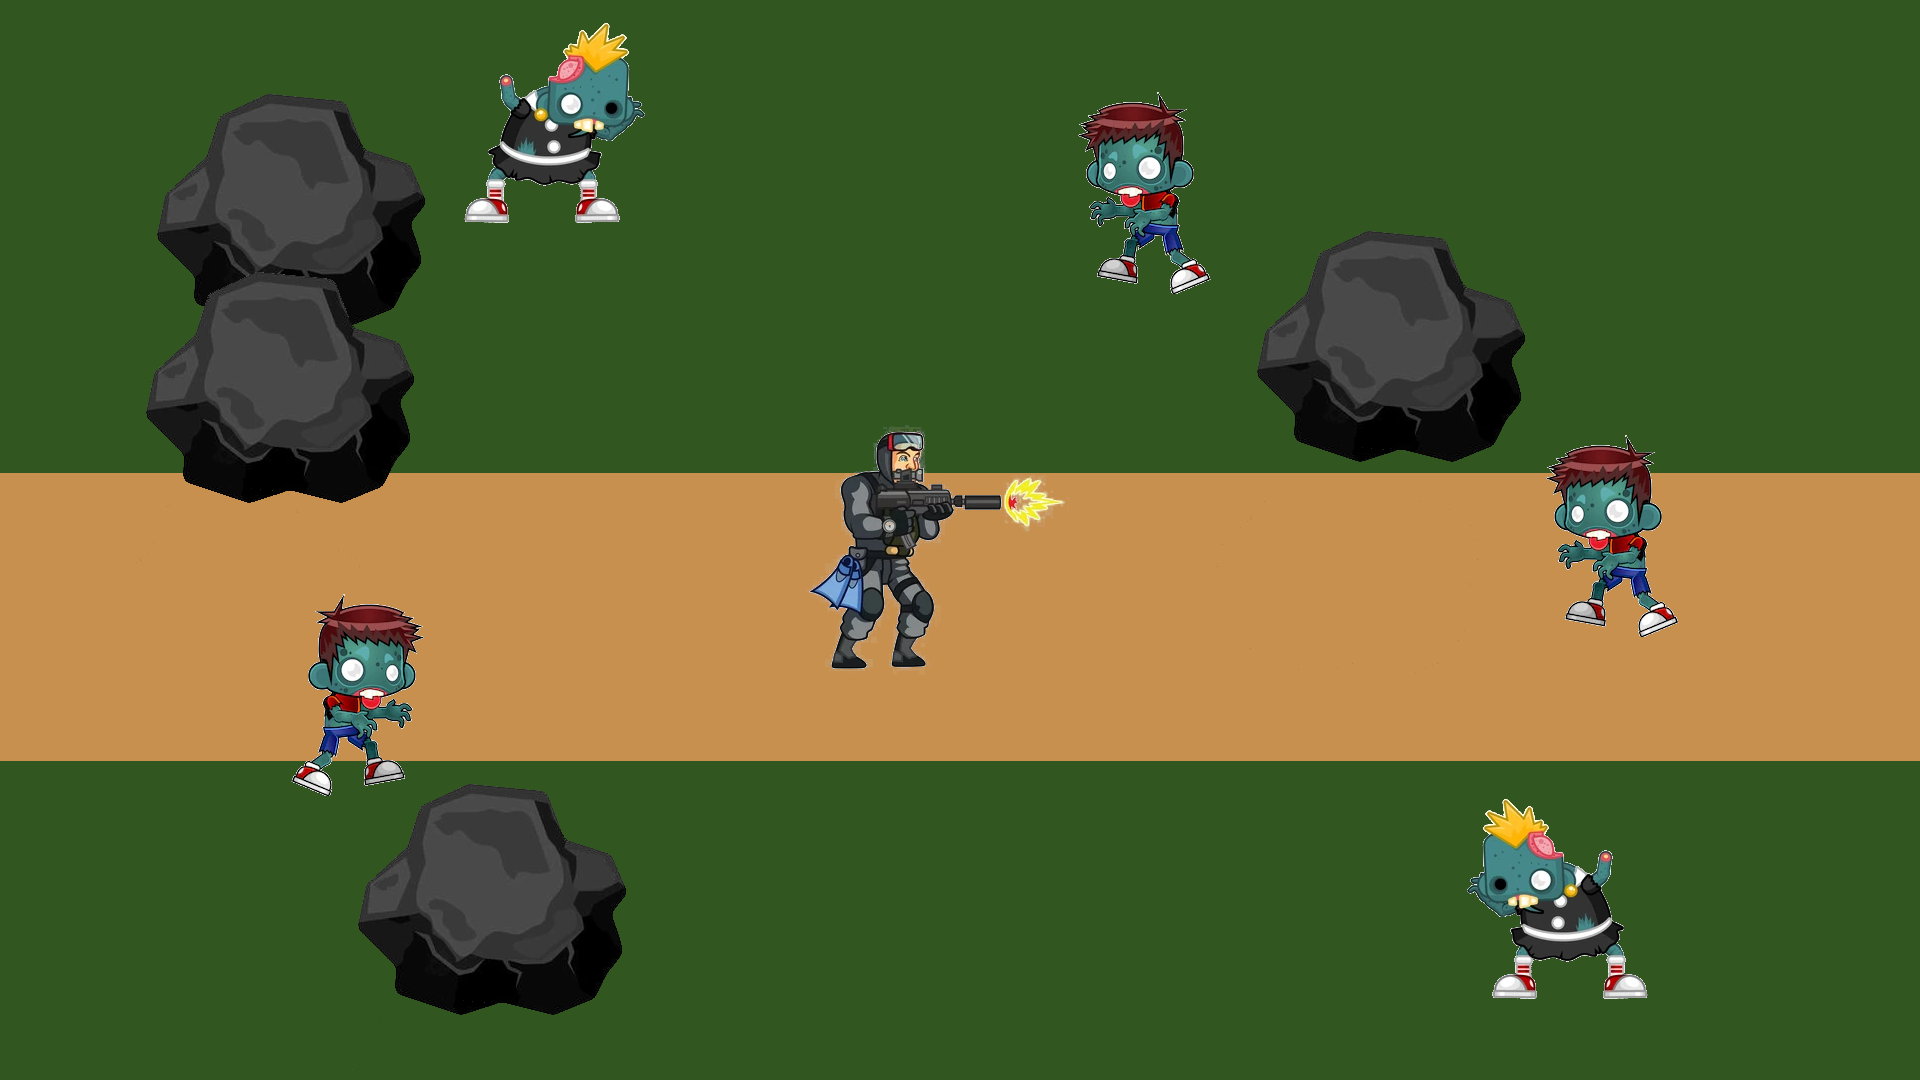
\includegraphics[width=\linewidth]{test.png}
    \caption {En prototypbild av spelet}
    \label {fig:picture}
  \end {figure}

  \section{Kravformulering}
  Nedan kommer det listas olika typer av krav, ska-krav är något som ska uppfyllas av spelet för att klara kursens mål. Bör-krav är något som inte nödvändigtvis behövs men kommer läggas till i spelet i mån av tid.
  \subsection{Ska-krav}
  \begin{enumerate}[label=S\arabic*]
    \item Spelaren ska med hjälp av piltangenterna kunna förflytta spelarkaraktären enligt tabell \ref{tab:movement}.
    \item Det ska finnas en fiende som attackerar på nära håll och en fiende som kan skjuta projektiler.
    \item Fienden ska förflytta sig mot spelaren.
    \item Om en fiende skjuter eller kolliderar med spelaren ska spelarens hälsa minska med hur mycket beroende på vilken fiende typ det var.
    \item Spelaren ska ha ett vapen som skjuter iväg en projektil.
    \item Om spelaren träffar fienden med en projektill ska fienden ta skada.
    \item När en fiende når 0 eller mindre i hälsa ska fiende försvinna från spelplanen.
    \item Om spelarens hälsa når 0 eller mindre ska spelet avslutas och game over visas.
    \item En tvådimensionell spelplan ska ritas ut på skärmen och ska täcka hela spelfönstret.
    \item Spelplanens uteseende slumpas fram, hinder och skydda hamnar på olika platser.
    \item En våg består av många olika fiender.
    \item När spelaren dödar en fiende ska poäng erhållas.
  \end{enumerate}

  \subsection{Bör-krav}
  \begin{enumerate}[label=B\arabic*]
    \item Det skall finnas en startmeny där spelaren kan välja att spela eller avsluta spelet.
    \item Startmenyn ska ha ett alternativ för att ändra keybindings.
    \item Vapen ska kunna uppgraderas.
    \item När spelaren dödar en fiende ska experience points erhållas.
    \item Fienden ska ha olika förflyttningsmönster.
    \item Det ska finnas olika typer av attacker för fienden.
    \item Det finns hinder som spelar- och fienden kan kollidera med.
  \end{enumerate}

  \section{Kravuppfyllelse}
  Nedan länkas våra ska-krav ovanför med krav från kursen så den enkelt går att se vilka av kraven på spelet uppfyller kraven från kursen.
  \addtocontents{toc}{\protect\setcounter{tocdepth}{0}}

  \subsection{Spelet ska simulera en värld som innehåller olika typer av objekt. Objekten ska ha olika beteenden och röra sig i världen och agera på olika sätt när de möter andra objekt.}
  Uppfylles av krav S1, S2, S3, S4, S6, S7, S8.
  \subsection{Det måste finnas minst tre olika typer av objekt och det ska finnas flera instanser av minst två av dessa. T.ex ett spelarobjekt och många instanser av två olika slags fiendeobjekt.}
  Uppfylles av krav S1, S2, S3, S11.
  \subsection{Ett beteende som måste finnas med är att figurerna ska röra sig över skärmen. Rörelsen kan följa ett mönster och/eller vara slumpmässig. Minst ett objekt, utöver spelaren ska ha någon typ av rörelse.}
  Uppfylles av krav S1, S3.
  \subsection{En figur ska styras av spelaren, antingen med tangentbordet eller med musen. Du kan även göra ett spel där man spelar två stycken genom att dela på tangentbordet (varje spelare använder olika tangenter). Då styr man var sin figur.}
  Uppfylles av krav S1.
  \subsection{Grafiken ska vara tvådimensionell.}
  Uppfylles av krav S9.
  \subsection{Världen (spelplanen) kan antas vara lika stor som fönstret (du kan göra en större spelplan med scrollning, men det blir lite krångligare).}
  Uppfylles av krav S9.
  \subsection{Det ska finnas kollisionshantering, det vill säga, det ska hända olika saker när objekten möter varandra, de ska påverka varandra på något sätt. T.ex kan ett av objekten tas bort, eller så kan objekten förvandlas på något sätt, eller så kan ett nytt objekt skapas. (Ett exempel på att skapa/ta bort objekt är när man i Space Invaders trycker på skjuta-knappen, t.ex en musknapp, då avfyras ett laserskott och skottet blir då en ny figur som skapas och placeras i världen, på en position vid laserkanonens mynning. Skottet rör sig framåt (uppåt) och om det träffar ett fiendeskepp tas både skottet och skeppet bort, om skottet kommer utanför spelplanen, dvs det missar, tas det endast bort.)}
  Uppfylles av krav S4, S6.
  \subsection{Det ska vara enkelt att lägga till eller ändra banor i spelet. Detta kan exempelvis lösas genom att läsa in banor från en fil (lite som i Sokoban-labben i TDP002), eller genom att ha funktioner i programkoden som bygger upp en datastruktur som definierar en bana.}
  Uppfylles av krav S10.
  \subsection{Spelet måste upplevas som ett sammanhängande spel som går att spela!}
  Uppfylles av alla krav.


\end{document}
